\documentclass[12pt, a4paper]{scrreprt}
\usepackage[utf8]{inputenc}
\usepackage[ngerman]{babel}
\usepackage[bookmarksnumbered]{hyperref}
\usepackage{graphicx}
\usepackage{keystroke} %Keyboardsymbole

\begin{document}
\begin{titlepage}
\titlehead{
	\begin{minipage}[c][5cm][c]{5cm}
	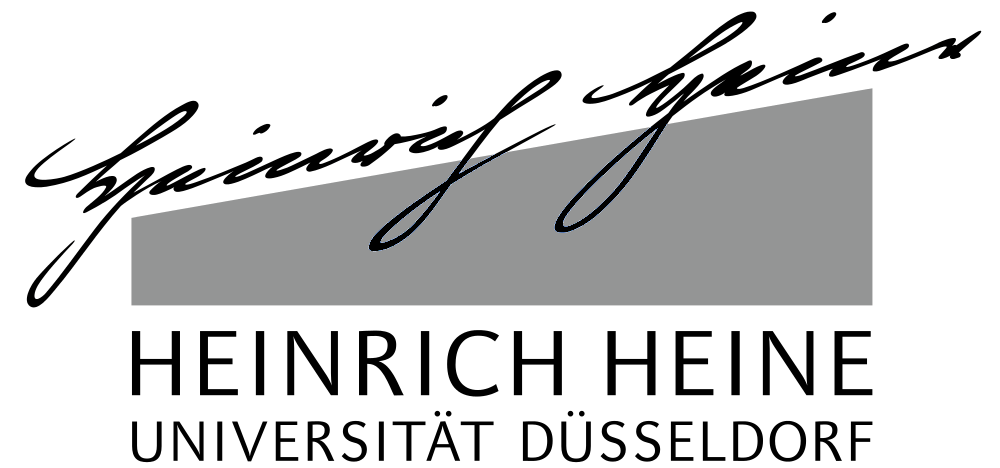
\includegraphics[width=48mm]{logo2}
	\end{minipage}
	\hfill
	\begin{minipage}[c][5cm][c]{10cm}
	\begin{flushright}
	\textbf{Universität Düsseldorf\\Mathematisch-Naturwissenschaftliche Fakultät\\Institut für Informatik\\Dozent:} PD Dr. Wilfried Linder
	\end{flushright}
	\end{minipage}
}
\subject{Benutzerhandbuch}
\title{Dungeon Crawler 	
	\begin{minipage}[c][1cm][c]{1cm}
	
\includegraphics[width=10mm]{Icon}
	\end{minipage}}
\subtitle{Programmierpraktikum im Sommersemester 2013}
\author{Michael Beurskens\\ Robin Thüs\\ Ruslan Curbanov}
\publishers{Gruppe 22}
\maketitle
\end{titlepage}
\tableofcontents
\chapter{Einleitung}
\section{Vorwort und Systemanforderungen}
\subsection*{Gesundheitsschutz}
\begin{itemize}
\item Legen Sie zum Schutz Ihrer Gesundheit eine Pause von 15 Minuten pro Spielstunde ein.
\item Spielen Sie nicht wenn Sie müde sind oder nicht genug Schlaf hatten.
\item Spielen Sie immer in einem gut beleuchteten Raum und setzen Sie sich so weit vom Bildschirm entfernt, wie es das Kabel Ihrer Eingabegeräte zulässt.
\item Bei einem sehr kleinen Prozentsatz von Personen kann es zu epileptischen Anfällen kommen, wenn sie bestimmten Lichteffekten oder Lichtmustern in ihrer täglichen Umgebung ausgesetzt sind.
\item Manchmal wird bei diesen Personen ein epileptischer Anfall ausgelöst, wenn sie Computerspiele spielen. Auch Spieler, die zuvor noch nie einen Anfall hatten, können an bisher nicht erkannter Epilepsie leiden. Falls Sie an Epilepsie leiden, suchen Sie Ihren Arzt auf, bevor Sie Computerspiele betreiben. Sollten bei Ihnen eines der folgenden Symptome auftreten (Schwindelgefühl, veränderte Sehkraft, Muskelzuckungen, jegliche Art von unkontrollierter Bewegung, Bewusstseinsverlust, Desorientierung und/oder Krämpfe), so brechen Sie das Spiel sofort ab und suchen einen Arzt auf.
\end{itemize}
\subsection*{Spielstart}
Vielen Dank, dass Sie sich für unsere neuste Entwicklung des Computerspiele-Zeitalters entschieden haben. Ich darf stolz verkünden, dass Sie mit diese Entscheidung eine hervorragende Wahl getroffen haben. Dungeon Crawler 2013 (Gruppe 22) wird nach unseren Prognosen das beliebteste Spiel des Jahres 2013!\\
\begin{enumerate}
\item Beachten Sie zunächst die Systemanforderungen, bevor Sie das Spiel Installieren.
\item Schalten Sie Ihren Computer ein und installieren das Spiel.
\item Starten Sie das Spiel mit \textit{Gruppe22.exe} (Server: \textit{DungeonServer.exe}).
\end{enumerate}
\subsection*{Systemanforderungen}
Bei der Entwicklung wurde besonders viel Wert auf Kompatibilität zu verschiedenen Geräten bzw. Systemen gelegt. Die hier zugrunde liegende Version ist jedoch nur unter Windows (ab XP bzw. unter .NET-Framework) lauffähig.\\
Beachten Sie: Das Spiel nutzt die Grafikbibliotheken \textit{OpenGL} (und \textit{OpenAL}), Ihre Grafikkarte sollte dies also unbedingt unterstützen.\\\\
Und sonst: Jedes halbwegs moderne Rechner tut's ;)
\section{Befehlsliste und Steuerung}
\textbf{\textit{Hinweis:}} Im folgenden wird mit dem Begriff \textit{Hauptmenü} das \textit{Pausenmenü} bezeichnet, da es sich in diesem GUI-System um das selbe Menü handelt.
\begin{center}
\begin{tabular}[here]{|l|l|}
\hline
Bewegen & \textit{Maus in Zielrichtung halten und linke Maustaste gedrückt halten}\\ \hline
Aktion & \textit{linke Maustaste drücken und halten (auf aktionsfähigem Objekt)}\\ \hline
Sekundärwaffe & \textit{Leertaste \Spacebar}\\ \hline
\multicolumn{2}{|c|}{Menüsteuerung und sonstige Befehle}\\ \hline
Pausenmenü & \Esc\\ \hline
Chat & \keystroke{T}\\ \hline
TODO & Ergänzen und vervollständigen!\\ \hline
\end{tabular}
\end{center}
\section{Prolog}

\section{Besetzung}
\section{Schauplätze}
\chapter{Einrichten des Spiels}
\section{Hauptmenü}
\begin{figure}[h]
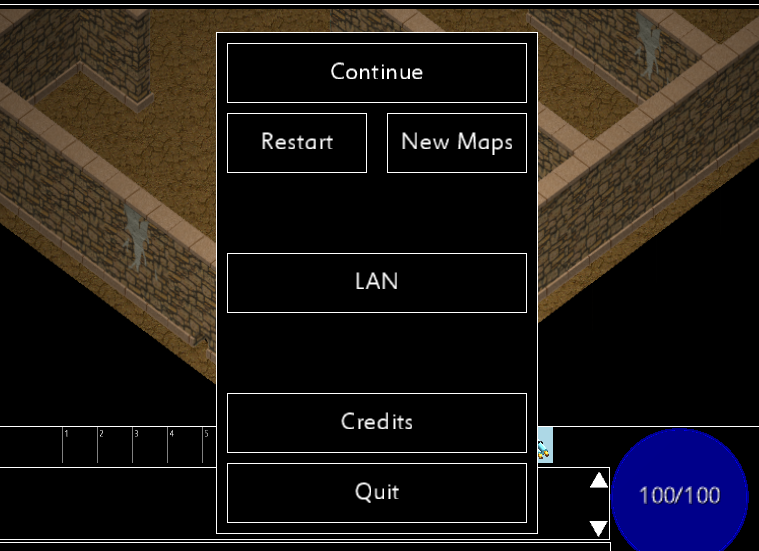
\includegraphics[width=\textwidth]{img/menu}
\caption{Hauptmenü des Spiels.}
\end{figure}
\section{Optionen}
\chapter{Gameplay und Anzeigesysteme}
\chapter{Multiplayer}
\section{Die Lobby}
\section{Das Chatsystem}
\chapter{Speichern und Laden}
\chapter{Lizenzbedingungen}
\chapter{Support}
\end{document}